
% !TeX spellcheck = de_DE
\documentclass{article}

\usepackage[ngerman]{babel}
\usepackage{graphicx}
\usepackage{indentfirst}
\usepackage{hyperref}
\usepackage{geometry}
\usepackage{changepage}

\graphicspath{ {./images/} }

\makeatletter
\newcommand{\sectionauthor}[1]{
	{\parindent 0em \large \scshape Autor: #1 \par \nobreak \vspace*{1em}}
	\@afterheading
}
\newcommand{\specification}[3]{
	{\parindent 0.5em \hangindent 3em \hypertarget{spec:#1:#2}{\textbf{/#1#2/}} #3 \par \nobreak \vspace*{0.5em}}
}
\makeatother

\begin{document}

%--Einleitung--------------------------------------------------------------------------------------------------------------------------------------------------------------------------
\section{Einleitung}
\sectionauthor{Jonas Picker}
Hier wird der Entwurf des Bibliotheksmanagementsystems BiBi beschrieben. Das Dokument bezieht sich auf das Lastenheft von Christian Bachmaier und Armin Größlinger und stellt eine technische Vertiefung unseres Pflichtenhefts dar, welches im Folgenden wiederholt referenziert wird. 

%--Systemarchitektur---------------------------------------------------------------------------------------------------------------------------------------------------------------
\section{Systemarchitektur}
\sectionauthor{Ivan Charviakou}

%--Klassendiagramm---------------------------------------------------------------------------------------------------------------------------------------------------------------
\section{Klassendiagramm}
\sectionauthor{Mohamad Najjar}

%--JSF-Dialoge-----------------------------------------------------------------------------------------------------------------------------------------------------------------------
\section{JSF-Dialoge}
\sectionauthor{León Liehr}


%--Systemfunktionen----------------------------------------------------------------------------------------------------------------------------------------------------------------
\section{Systemfunktionen}
\sectionauthor{Jonas Picker}
\subsection{Technische Systemsicherheit}
\noindent \textbf{Kommunikationserschlüsselung:} Durch die CA-Zertifizierung des Servers wird eine TLS-Transportverschlüsselung bei der Kommunikation zwischen Klient und Server verwendet. Ist die Datenbank, wie im Abschnitt 4.3  'Server' beschrieben, über SSL-VPN angebunden, ist die Kommunikation zwischen ihr und dem Server ebenfalls verschlüsselt. \\
\textbf{Nutzerberechtigungen:} Für die Überprüfung der Zugangsberechtigungen bei jeder HTTPS-Anfrage implementiert die Klasse !!!!!!!!!!!!!!!!!!!!!!!!!!!!!!!!!!!\hyperlink{}{} das PhaseListener-Interface, welches zu implementierende Methoden zum Ausführen von Code vor oder nach jeder Phase des JSF-Life-Cycle vorgibt. In unserem Fall wird am frühestmöglichen Punkt (vor der Restore-View-Phase) geprüft, ob der Anfragesteller auch berechtigt ist, die vorhergesehene Antwort vom Server zu erhalten. Aus Redundanzgründen verwenden wir für Seiten, auf die mehrere Nutzerrollen Zugriff haben, die gleichen Facelets. In den jeweiligen Backing-Beans wird dann, durch Zugriff auf die von JSF getrackte Nutzer-Session der Klasse  !!!!!!!!!!!!!!!!!!!!!!!!!!!!!!!\hyperlink{}{}, die Rolle des Benutzers überprüft. Durch die inklusive Rollenhierarchie lassen sich so alle Funktionalitäten der Rollen im gleichen Facelet einbinden.\\
\textbf{Session-Hijacking\footnote{Das Stehlen einer validen Nutzer-Session um Zugriff auf den Account und seine Berechtigungen zu erhalten}:} Es wird durch das manuelle Austauschen des Identifikators für die Nutzer-Session an kritischen Stellen dafür gesorgt, dass Session-Hijacking unmöglich wird. \\
\textbf{Cross-Site-Scripting\footnote{Einschleusen von browserinterpretierbarem HTML-Code auf ungesicherte Teile einer Website}:} Alle Elemente der JSF-Facelets, die nutzergenerierten In- und Output weitergeben, haben den impliziten Standartwert 'escape=true'. Da wir diesen in unserer Implementierung nie manuell auf 'false' setzen, greift das JSF-interne Escapen von HTML-Sonderzeichen bei allen nutzergenerierten Teilen der Anwendung. \\
\textbf{SQL-Injection\footnote{Einschleusen von SQL-Code in Formularfelder, um Zugriff auf die Datenbank zu erhalten}:} Durch das Konsequente Verwenden der 'Prepared Statements' in unserer !!!!!!!!!!!!!!!!!!!!!!!!!!!!!!!!!!!!\hyperlink{}{Datenzugriffsschicht} beugen wir SQL-Injections vor. Diese JDBC-Funktionalität trennt das eigentliche SQL-Statement von den nutzergenerierten Parametern und Verhindern so das Ausführen von maliziösem SQL-Code in der Datenbank. \\
\subsection{Logging}
Mit der Klasse !!!!!!!!!!!!!!!!!!!!!!!!!!!!!!\hyperlink{}{} ist unser System mit einer eigenen Log-Funktion ausgestattet. Diese dient sowohl zum Debugging während der Entwicklung, alsauch zum Protokollieren der Fehler und Abläufe im laufenden System. Durch Setzten der Variable 'LOG\_CONSOLE: ' mit den Werten 'TRUE' oder 'FALSE' kann eingestellt werden, ob die Meldungen auch in Echtzeit auf der Konsole ausgegeben oder nur in das Log-File geschrieben werden. Es gibt drei Log-Level, zwischen denen durch Setzen der Variable 'LOG\_LEVEL: ' in der Konfigurationsdatei mit einem der unten aufgeführten Werte beim Systemstart umgeschaltet werden kann. Die folgenden Kategorien sind inklusiv, die Letzte schließt somit die oberen beiden mit ein. \\
\textit{'SEVERE':} Diese Einstellung des Loggers protokolliert nur schwere Fehler, die unmittelbare Konsequenzen für den Anwendungsbetrieb haben. Um ein schnelles Volllaufen des Log-Files zu vermeiden, ist dies die Standarteinstellung.\\
\textit{'DETAILED':} Fehler und fehlgeschlagene Prozeduren, die die Integrität der Anwendung nicht gefährden (z.B. !!!!!!!!!!!!!!!!!!!!!!!!!!!!!\hyperlink{}{wie hier}) werden zusätzlich protokolliert.\\
\textit{'DEVELOPMENT':} Hierunter fallen sowohl Protokollierungen von erfolgreichen oder seltenen Abläufen, alsauch sonstige nützliche Meldungen. Da das Log-File schnell sehr groß und unübersichtlich werden könnte, empfehlen wir, diese Option nur bei Problemen zu wählen.\\
\subsection{Selbstständige Abläufe}
Die Klasse !!!!!!!!!!!!!!!!!!!!!!!!!!!!!!!!!!!!\hyperlink{}{} ermöglicht dem System, selbstständig in einstellbaren Abständen Wartungsaufgaben durchzuführen. Alle unten aufgelisteten Aufgaben sind somit von der der aktuellen Systemzeit des Servers abhängig und werden darüberhinaus nur mit einer maximalen zeitlichen Unsicherheit des gewählten Intervalls durchgeführt. Die Einstellung wird beim Systemstart durch den gesetzten Wert der Variable 'SCAN\_INTERVAL: ' bestimmt. Der von uns empfohlene Standartwert repräsentiert eine Minute, sollten Sie diesen verlängern wollen tragen Sie stattdessen eine andere positive ganze Zahl ein. Der Wartungsthread vergleicht die Operationsfrist der zur Abholung markierten Exemplare mit der aktuellen Systemzeit und setzt bei Überschreitung den Verfügbarkeitsstatus wieder auf 'verfügbar'. Bei Exemplaren mit dem Status 'ausgeliehen' wird, zusätzlich zur Frist, die Mahnungsversatzzeit beachtet und bei Bedarf die Klasse !!!!!!!!!!!!!!!!!!!!\hyperlink{}{} zum Versenden einer E-Mail angestoßen. Die abgelaufenen Tokens der Benutzer-Tabelle werden ebenfalls gelöscht.
\subsection{Datenbankverbindung}
Wenn die Java Laufzeitumgebung des Systems plötzlich beendet wird und das System abstürzt, wird mittels einer ShutdownHook trotzdem noch das Schließen offener Datenbankverbindungen versucht. Außerdem wird durch das logische Kapseln der voneinander abhängigen Datenbanktransaktionen durch die Klasse !!!!!!!!!!!!!!!!!!!\hyperlink{}{} sichergestellt, dass das ACID-Prinzip bestmöglich eingehalten und die Datenbank im Fehlerfall in einem konsistenten Zustand hinterlassen wird. Dies ist jedoch (z.B. bei einem Stromausfall) nicht immer möglich.
\subsection{Starten und Stoppen der Anwendung}
\noindent \textbf{Start:} Durch Implementierung des SystemEventListener-Interface werden beim Systemstart von der Klasse !!!!!!!!!!!!!!!!!!!!!!!!!!!\hyperlink{}{} alle weiteren Aktionen angestoßen. Die Initialisierung des !!!!!!!!!!!!!!!!!!!!!!!!!!!!!!!!!!!!\hyperlink{}{Loggers} geschieht zuerst, danach wird die Konfigurationsdatei eingelesen, das Log-Level gessetzt und mit den restlichen Parametern eine !!!!!!!!!!!!!!!!!!!!!!!!!!\hyperlink{}{eigene Initialisierungsklasse} für Prozesse der !!!!!!!!!!!!!!!!!!!!\hyperlink{}{Buisnesslogik/Serviceschicht} aufgerufen. Diese wiederum gibt die Initialisierung der !!!!!!!!!!!!!!!!!!!!!!!!!!!!!!!!!!!!\hyperlink{}{Datenzugriffsschicht} an eine !!!!!!!!!!!!!!!!!!!!!!!!!!!!\hyperlink{}{weitere Klasse} ab, in der zunächst die Datenbankverbindung überprüft wird. Sollten die Verbindung fehlschlagen, wird !!!!!!!!!!!!!!!!!!!\hyperlink{}{eine Fehlermeldung} ausgegeben/geloggt. Im Erfolgsfall wird dann überprüft, ob die benötigten Tabellenstrukturen bereits vorhanden sind. Falls nicht wird das manuelle Anlegen der Tabellen (Mediumsschema wird mit !!!!!!!!!!!!!!!!!!!!!!!\hyperlink{}{Default} befüllt) über einen Konsoleninput mit 'Y' oder 'N' entschieden werden müssen. Bei existierenden Tabellen wird  nun der !!!!!!!!!!!!!!!!!!\hyperlink{}{Connection-Pool} initialisiert und der Startprozess der !!!!!!!!!!!!!!!!!!!!!!!!!!!!!!!!!!!!\hyperlink{}{Datenzugriffsschicht} ist abgeschlossen. Es wird die  !!!!!!!!!!!!!!!!!!!!\hyperlink{}{darüberliegende Schicht} benachrichtigt und von !!!!!!!!!!!!!!!!!!!!!!!!!!!\hyperlink{}{dort} aus der !!!!!!!!!!!!!!!!!!\hyperlink{}{Wartungsthread} aktiviert. Die nun folgende Erfolgsmeldung zurück an den !!!!!!!!!!!!!!!!!!!!!!!!!!!\hyperlink{}{SystemEventListener} gibt das momentan ausgewählte Farbschema nach oben durch, danach ist das System betriebsbereit. \\
\textbf{Stop:} 
Beim planmäßigen Herunterfahren des Systems durch das Ausschalten des Tomcat auf dem Server (z.B. via shutdown.sh) reicht der !!!!!!!!!!!!!!!!!!!!!!!!!!!\hyperlink{}{SystemEventListener} eine Nachricht an die Klasse!!!!!!!!!!!!!!!!!!\hyperlink{}{}, von wo aus zunächst der !!!!!!!!!!!!!!!!!!\hyperlink{}{Wartungsthread} beendet und danach die !!!!!!!!!!!!!!!!!!!!!!!!!!!!!!!!!!!!\hyperlink{}{Datenzugriffsschicht} kontaktiert wird. Von !!!!!!!!!!!!!!!!!!!!!!!!!!!\hyperlink{}{dort} aus werden zunächst die noch offenen Datenbankverbindungen über den !!!!!!!!!!!!!\hyperlink{}{Connection-Pool} geschlossen und, nach Durchreichen der Erfolgsmeldung nach oben, die Anwendung gestoppt. Nutzersessions überleben das Ausschalten des Servers nicht.
%--Datenfluss--------------------------------------------------------------------------------------------------------------------------------------------------------------------------
\section{Datenfluss}
\sectionauthor{Sergei Pravdin}

%--ER-Modell--------------------------------------------------------------------------------------------------------------------------------------------------------------------------
\section{ER-Modell}
\sectionauthor{Jonas Picker}

\newgeometry{left=0cm,right=0cm,top=0cm,bottom=0cm}

\begin{figure}[h]
    \centering
    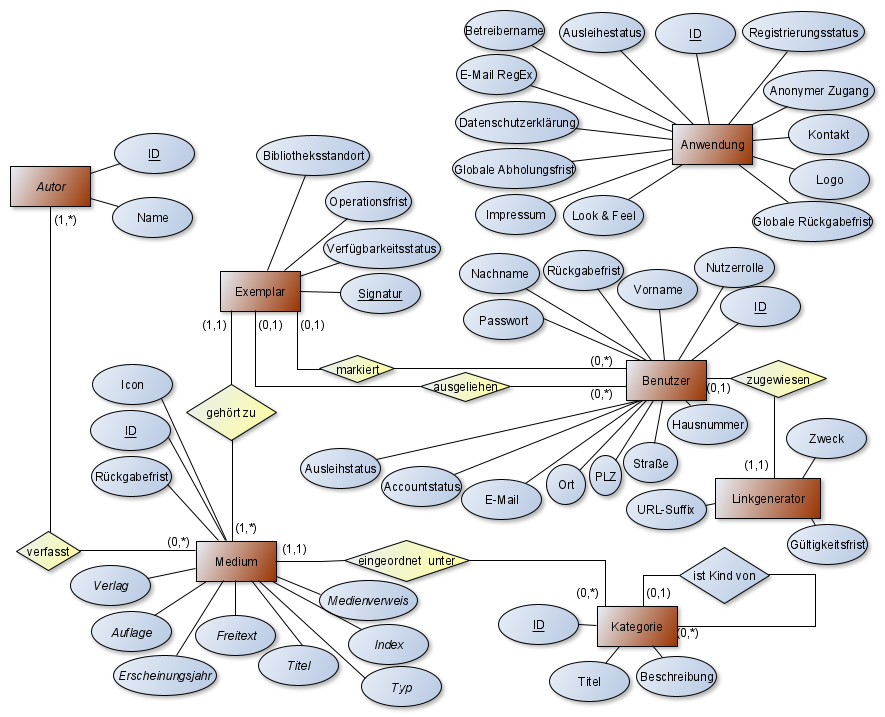
\includegraphics[angle = 270, width = 60em]{ER-Diagramm}
    \caption{Entity-Relationship Diagramm}
    \label{ER-Diagramm}
\end{figure}

\restoregeometry
\newpage

\subsection{Legende}
Jede Entität wird im Folgenden zusammen mit ihren nicht offensichtlichen Attributen und Relationen kurz beschrieben.\\
\textbf{Medium:} Diese Entität modelliert die in der Bibliothek gehaltenen Medien. Zusätzlich zum Primär-schlüssel ist auch das Attribut 'Rückgabefrist' und 'Icon' nicht vom Administrator entfernbar, die restlichen Attribute (kursiv) stellen den modifizierbaren Standartsatz der Medienattribute dar (PfHft. /D020/). Erwähnenswert ist hier noch das als mehrwertig markierte, editierbare Attribut 'Autoren', diese Markierung kann auch zu benutzerdefinierten Attributen hinzugefügt werden und wird mit dem Anlegen einer neuen Entität modelliert (PfHft. /F380/).\\
\textbf{Kategorie:} Die mit dieser Entität verbundenen Relationen ordnen jedem Medium genau eine Kategorie zu und modellieren die Kategoriehierarchie (PfHft. /W440/) durch die Selbstbeziehung. Es wird einen unlöschbaren Top-Knoten in der Hierarchie geben, zu dem alle Medien, die nie in eine Kategorie eingeteilt wurden oder deren Kategorie gelöscht wurde, gehören. Sollten alle Medien in benutzerdefinierten Kategorien stecken, hat der Top-Knoten keine zugeordneten Medien und nimmt somit nicht an der 'eingeordnet unter'-Relation teil.\\
\textbf{Exemplar:} Von jedem Medium muss mindestens ein Exemplar vorhanden sein. Auch kann ein bestimmtes Exemplar von genau einem Nutzer zur Abholung markiert oder ausgeliehen werden, diese Aktionen schließen sich gegenseitig aus (PfHft. /F310/) und ändern (genau wie eine Rückgabe) den Verfügbarkeitsstatus und die dazugehörige Operationsfrist dementsprechend. \\
\textbf{Benutzer:} Ob ein Benutzer die Ausleihfunktion benutzen kann, wird durch das Attribut 'Ausleihstatus' modelliert. 'Accountstatus' zeigt hingegen an, ob der Nutzeraccount bereits den Verifizierungsprozess durchlaufen hat (PfHft. /W70/). Das Passwort wird in gehashter Form abgespeichert. \\
\textbf{Linkgenerator:} Diese Entität kapselt einen befristet gültigen URL-Suffix, aus dem der Verifizierungs- oder Passwortzurücksetzungslink (je nach Zweck) für genau einen Account erstellt wird.\\
\textbf{Anwendung:} Hier werden die setzbaren globalen Variablen und Anwendungseinstellungen gespeichert. Diese Tabelle hat nur einen einzigen Eintrag. 'Anonymer Zugang' modelliert die Berechtigungen anonymer Nutzer beim Besuchen des Webspaces (PfHft. /F10/), während 'Registrierungsstatus' eine nutzerfreundlichere Alternative als den RegEx zum Sperren der Registrierung bietet (PfHft. /F20/). 'Ausleihstatus' steht für das Umschalten des Systems zur manuellen Freischaltung der Ausleihfunktion für registrierter Nutzer. 'Look \& Feel' speichert das momentan ausgewählte Farbschema. \\

\end{document}

